\chapter{Team Declaration \\
\small{\textit{-- Chan, Moks, Ponte}}
\index{team declaration} 
\index{Chapter!Team Declaration}
\label{Chapter::Team Declaration}}

\section*{Project Proposal}
Our project focuses on developing a secure, user-friendly translation framework that enables non-experts to leverage the power of quantum optimization. Specifically, we aim to build upon recent research in natural language interfaces for quantum computing by designing a modular, object-oriented system that translates high-level problem descriptions into Quadratic Unconstrained Binary Optimization (\gls{QUBO}) models suitable for execution on quantum solvers. 

The proposed platform bridges the gap between everyday users and complex quantum technologies by providing an intuitive, natural language interface enhanced with validation, error detection, and semantic verification. By integrating object-oriented principles, we intend to improve system maintainability, scalability, and extensibility while ensuring that the translation process remains trustworthy and efficient. Our long-term vision is to create a framework that can be expanded beyond academic use to practical applications in logistics, scheduling, and resource allocation.

\section*{Mission Statement}
The mission of our project is to lower the barrier to quantum computing adoption by creating a reliable natural language interface that translates optimization problems into \gls{QUBO} formulations. This addresses the business need for organizations to explore quantum computing without requiring specialized expertise, while also supporting the business intent of enabling faster, more efficient decision-making processes in industries such as transportation, healthcare, and operations management.


\section*{Key Drivers}
Several factors motivate the pursuit of this project:  

1. \textbf{Accessibility to Quantum Computing:} Currently, most quantum programming requires advanced mathematical and technical skills, creating a steep learning curve. By designing an intuitive natural language interface, we aim to make quantum optimization accessible to researchers, students, and professionals outside of quantum physics or computer science.  

2. \textbf{Growing Business Demand:} Organizations across industries face increasingly complex optimization challenges such as delivery routing, workforce scheduling, and network design. Quantum computing offers promising solutions, but adoption is limited by the lack of approachable tools. Our project addresses this need by providing a bridge between user intent and quantum execution.  

3. \textbf{Verification and Trustworthiness:} Large language models (\gls{LLM}), while powerful, are prone to errors such as hallucination or structural inconsistencies. To ensure real-world applicability, our system introduces safeguards like schema validation, reverse translation, and semantic \gls{fidelity} scoring. These features directly enhance trustworthiness, which is critical for industries where correctness and reliability cannot be compromised.  

4. \textbf{Educational Value:} Beyond immediate applications, our platform serves as a learning tool to help students and professionals understand the relationship between high-level problem descriptions and quantum-ready models. This educational aspect expands the reach and long-term sustainability of the system.  


\section*{Key Constraints}
Despite its potential, our project must operate within several constraints:  

1. \textbf{Resource Limitations:} Access to true quantum hardware (such as D-Wave annealers) is limited and expensive. As a result, our system will initially rely on simulators or cloud-based quantum services. This constraint requires us to optimize for efficiency, ensuring that the translation pipeline works reliably even with limited compute resources.  

2. \textbf{LLM Reliability:} Large language models can produce inconsistent or incorrect outputs depending on the prompt or problem complexity. To address this, our design must incorporate multiple validation layers and fallback mechanisms, but we recognize that absolute accuracy cannot be guaranteed. This constraint influences how we evaluate success and measure system robustness.  

3. \textbf{Complexity of Optimization Problems:} Not all optimization problems translate neatly into QUBO formulations. Problems involving intricate relational constraints may cause higher failure rates. This constraint drives us to focus on representative problem sets while gradually expanding to more challenging categories.  

4. \textbf{Time and Scope:} As an academic project with a defined timeline, we must balance ambition with feasibility. While future work could include fine-tuning models or integrating with symbolic verification tools, our current milestone limits us to replicating and incrementally improving the existing framework.  

Together, these constraints frame our project as both ambitious and pragmatic. By acknowledging them early, we position our team to deliver a functional, professional-grade prototype that demonstrates both technical feasibility and meaningful improvement upon prior work.

\section{Background and Prior Work}

Last year’s group introduced the idea of a trustworthy natural language interface for quantum optimization, focusing on translating user prompts into structured \gls{JSON} representations. Their system leveraged large language models to generate decision variables, constraints, and objectives, and they evaluated these outputs with schema validation to determine structural correctness. They tested across five canonical problem types—Knapsack, Traveling Salesman Problem (TSP), Graph Coloring, Seating Assignment, and Team Assignment—measuring success rates, failure categories, and latency. This work demonstrated that GPT-4 outperformed GPT-3.5 on several problems, achieving higher rates of schema-valid JSON and maintaining interactive performance times.

However, the prior group’s implementation never extended beyond JSON validation. They did not complete the reverse translation step that compares the generated \gls{QUBO} representation back to the original prompt for semantic fidelity. They also did not translate the validated JSON into QUBO form or run it on a quantum solver, leaving critical components of the proposed framework unimplemented. As a result, their evaluation was limited to whether JSON outputs were well-formed, without testing true semantic alignment or solver compatibility.

Our project builds directly on this foundation by addressing these gaps. Specifically, we are working to (i) implement reverse translation and fidelity scoring so that semantic accuracy can be quantitatively measured, (ii) translate valid JSON outputs into executable QUBO formulations, and (iii) extend the system with modular, object-oriented components for maintainability and scalability. By completing these steps, our goal is to move beyond structural validation and establish a pipeline that not only produces valid JSON but also ensures semantic correctness and quantum-executable outputs.

\section{System Architecture}

\begin{figure}[H]
    \centering
    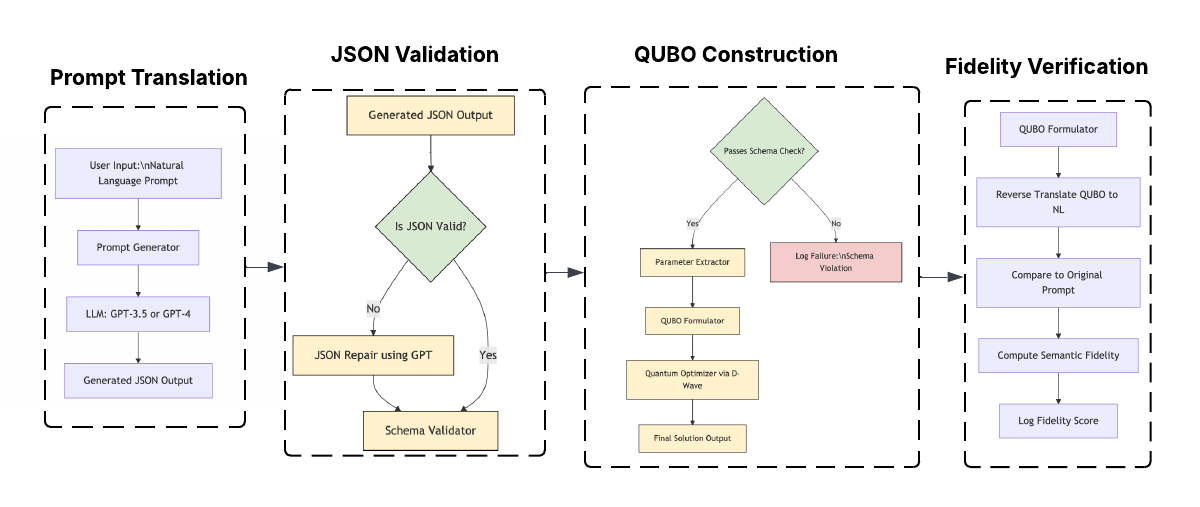
\includegraphics[width=.9\linewidth]{png/QSEC-2.png}
    \caption{LLM-to-QUBO Pipeline Architecture}
    \label{fig:Pipeline}
\end{figure}